\documentclass[a4paper,12pt, oneside]{book}

% \usepackage{fullpage}
\usepackage[italian]{babel}
\usepackage[utf8]{inputenc}
\usepackage{amssymb}
\usepackage{amsthm}
\usepackage{graphics}
\usepackage{amsfonts}
\usepackage{listings}
\usepackage{amsmath}
\usepackage{amstext}
\usepackage{engrec}
\usepackage{rotating}
\usepackage{verbatim}
\usepackage[safe,extra]{tipa}
% \usepackage{showkeys}
\usepackage{multirow}
\usepackage{hyperref}
\usepackage{microtype}
\usepackage{fontspec}
\usepackage{enumerate}
\usepackage{physics}
\usepackage{braket}
\usepackage{marginnote}
\usepackage{pgfplots}
\usepackage{cancel}
\usepackage{polynom}
\usepackage{booktabs}
\usepackage{enumitem}
\usepackage{framed}
\usepackage{pdfpages}
\usepackage{pgfplots}
\usepackage{algorithm}
% \usepackage{algpseudocode}
\usepackage[cache=false]{minted}
\usepackage{mathtools}
\usepackage[noend]{algpseudocode}
\newcommand*{\bfrac}[2]{\genfrac{}{}{0pt}{}{#1}{#2}}

\usepackage{tikz}\usetikzlibrary{er}\tikzset{multi  attribute /.style={attribute
    ,double  distance =1.5pt}}\tikzset{derived  attribute /.style={attribute
    ,dashed}}\tikzset{total /.style={double  distance =1.5pt}}\tikzset{every
  entity /.style={draw=orange , fill=orange!20}}\tikzset{every  attribute
  /.style={draw=MediumPurple1, fill=MediumPurple1!20}}\tikzset{every
  relationship /.style={draw=Chartreuse2,
    fill=Chartreuse2!20}}\newcommand{\key}[1]{\underline{#1}}
\usetikzlibrary{arrows.meta}
\usetikzlibrary{decorations.markings}
\usetikzlibrary{arrows,shapes,backgrounds,petri}
\tikzset{
  place/.style={
    circle,
    thick,
    draw=black,
    minimum size=6mm,
  },
  transition/.style={
    rectangle,
    thick,
    fill=black,
    minimum width=8mm,
    inner ysep=2pt
  },
  transitionv/.style={
    rectangle,
    thick,
    fill=black,
    minimum height=8mm,
    inner xsep=2pt
  }
} 
\usetikzlibrary{automata,positioning,chains,fit,shapes}
\usepackage{fancyhdr}
\pagestyle{fancy}
\fancyhead[LE,RO]{\slshape \rightmark}
\fancyhead[LO,RE]{\slshape \leftmark}
\fancyfoot[C]{\thepage}
\usepackage[usenames,dvipsnames]{pstricks}
\usepackage{epsfig}
\usepackage{pst-grad} % For gradients
\usepackage{pst-plot} % For axes
\usepackage[space]{grffile} % For spaces in paths
\usepackage{etoolbox} % For spaces in paths
\makeatletter % For spaces in paths
\patchcmd\Gread@eps{\@inputcheck#1 }{\@inputcheck"#1"\relax}{}{}
\makeatother
\usepackage{lipsum}
\DeclareSymbolFont{symbolsC}{U}{txsyc}{m}{n}
\DeclareMathSymbol{\strictif}{\mathrel}{symbolsC}{74}
\title{Data Science Lab in Biosciences}
\author{UniShare\\\\Davide Cozzi\\\href{https://t.me/dlcgold}{@dlcgold}}
\date{}

\pgfplotsset{compat=1.13}
\begin{document}
\maketitle

\definecolor{shadecolor}{gray}{0.80}
\setlist{leftmargin = 2cm}
\newtheorem{teorema}{Teorema}
\newtheorem{definizione}{Definizione}
\newtheorem{esempio}{Esempio}
\newtheorem{corollario}{Corollario}
\newtheorem{lemma}{Lemma}
\newtheorem{osservazione}{Osservazione}
\newtheorem{nota}{Nota}
\newtheorem{esercizio}{Esercizio}
\algdef{SE}[DOWHILE]{Do}{doWhile}{\algorithmicdo}[1]{\algorithmicwhile\ #1}
\tableofcontents
\renewcommand{\chaptermark}[1]{%
  \markboth{\chaptername
    \ \thechapter.\ #1}{}}
\renewcommand{\sectionmark}[1]{\markright{\thesection.\ #1}}
\newcommand{\floor}[1]{\lfloor #1 \rfloor}
\newcommand{\MYhref}[3][blue]{\href{#2}{\color{#1}{#3}}}%
\chapter{Introduzione}
\textbf{Questi appunti sono presi a lezione. Per quanto sia stata fatta
  una revisione è altamente probabile (praticamente certo) che possano
  contenere errori, sia di stampa che di vero e proprio contenuto. Per
  eventuali proposte di correzione effettuare una pull request. Link: }
\url{https://github.com/dlcgold/Appunti}.\\
\chapter{Big Data in Biotechnology \& Biosciences}
\chapter{Making Sense of Biological Data}
La \textbf{biologia} è una \textit{scienza della vita} che include:
\begin{itemize}
  \item zoologia
  \item citologia
  \item ecologia
  \item botanica
  \item microbiologia
  \item fisiologia
  \item genetica
  \item biochimica
  \item $\ldots$
\end{itemize}
Tale scienza si occupa di capire le strutture, le funzioni, le origini, le
interazioni e la tassonomia (ovvero della classificazione) delle creature
viventi, non solo dell'uomo.\\
Si hanno vari livelli d'informazione con tanti approcci per lo studio delle
informazioni stesse. È come se avessi un enorme \textit{grafo multilayer} di
informazioni, molto \textit{complesso}. In questa scienza non si hanno regole
universali, si ha sempre l'eccezione. La validità dei metodi analitici dipende
fortemente da caratteristiche, conosciute o meno, dei dati stessi. Alcuni
algoritmi hanno sunti diversi a seconda della tipologia del dato biologico. I
dati sono tendenzialmente poco conosciuti. La \textit{biologia} prevede quindi
studi davvero molto complicati, più di quanto sembri. Inoltre alcuni fenomeni
sono difficilissimi da misurare e hanno una grande incertezza.\\ 
Si ha una \textit{struttura gerarchica evoluzionaria della biologia} ma solo
perché l'uomo ha strutturato le conoscenze sulla tassonomia. In realtà la vita è
meno schematica e più ``fluida'' di quel che si vuole credere. Si hanno quindi:
\begin{itemize}
  \item raggruppamento di specie simili
  \item specie 
  \item popolazione
  \item organismi
\end{itemize}
Un'altra gerarchia si basa sui fenomeni che interconnettono i vari livelli
appena elencati. Si hanno quindi i cosiddetti \textbf{ecosistemi}, avendo una
\textit{gerarchia ecologica}. Per l'uomo si
ha una \textit{reale}, ovvero dove vive un organismo, praticamente globale,
vivendo praticamente ovunque. Si hanno quindi interazioni tra queste varie
gerarchie nella biologia, che descrive sia le caratteristiche evolutive che
ambientali, come visibile in figura \ref{fig:ger}. \\
\begin{figure}
  \centering
  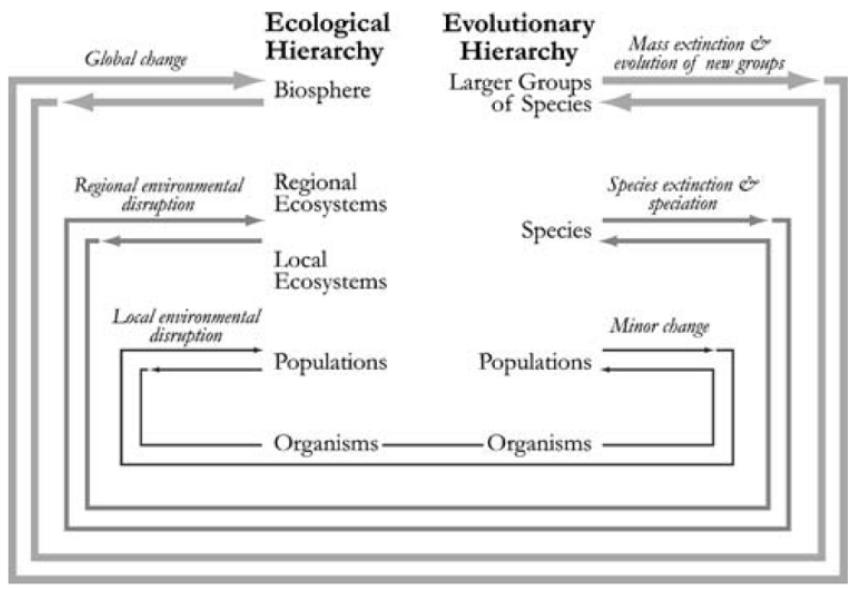
\includegraphics[scale = 0.4]{img/ger.jpg}
  \caption{Vecchio schema grafico delle gerarchie in biologia e delle loro
    interazioni.}
  \label{fig:ger}
\end{figure}
La biologia inoltre evolve molto in fretta anche nel definire i suoi formalismi
e i suoi limiti. Le pubblicazioni ``invecchiano'' molto in fretta.\\
In biologia si hanno delle \textit{regole}, influenzate comunque dalla
percezione umana che crea dei \textit{bias descrittivi} che si ripercuotono sui
dati stessi. Anche in questo le nuove tecnologie di sequenziamento permettono di
avere dati migliori, in quanto permettono di osservare il fenomeno in modo
corretto. 
\end{document}

% LocalWords:  clock  evoluzionaria
